\documentclass[french, a4paper, 12pt]{article}

%French setting up
\usepackage[utf8]{inputenc}
\usepackage[T1]{fontenc}
\usepackage{babel}

\setlength{\parindent}{0cm}
\usepackage{amsmath}
\usepackage{siunitx} %physics units
\usepackage{graphicx} % Images
\graphicspath{ {./images_chem/} }
\usepackage{fancyhdr}
\usepackage{float}
\usepackage[version=4]{mhchem} %Chemical equations

%Border
\usepackage[left=1in, right=1in, top=1in, bottom=1in]{geometry}
 
\pagestyle{fancy}
\fancyhf{}
\rhead{ImmortalPharaoh7}
\lhead{Notes de Révision Chimie NM}
\cfoot{\thepage}

\author{ImmortalPharaoh7}
\title{Notes de Révision Chimie NM}
\date{Mai 2020}

\usepackage{hyperref} %Last package
\urlstyle{same}
\begin{document}
\begin{titlepage}
\maketitle
\begin{abstract}
Les notes de révision pour la chimie niveau moyen du BI, pour le curriculum qui commence dès 2016. Attention, ces notes ne sont pas à être utilisées indépendamment; ils servent comme des astuces ou bien les définitions qui peuvent être oubliées.

Si vous avez des informations à ajouter ou bien des corrections, veuillez envoyer un email à pharaoh.immortal7@gmail.com ou messager ImmortalPharaoh7\#7811 sur Discord.
\end{abstract}
\end{titlepage}

\pagenumbering{roman}
\tableofcontents
\pagebreak

\pagenumbering{arabic}

\section{Relations Stœchiométriques}
\pagebreak

\section{Structure Atomique}
\pagebreak

\section{Périodicité}
\pagebreak

\section{Liaison et Structure Chimique}
\pagebreak

\section{Thermochimie}
\textbf{Définitions:}
\begin{itemize}
\item Enthalpie: Énergie emmagasinée dans un matériel.
\item Endothermique: Une réaction qui absorbe de l'enthalpie $\Delta H > 0$.
\item Exothermique: Une réaction qui libère de l'enthalpie $\Delta H < 0$.
\item Conditions standards: Température de \SI{298}{K} et pression de \SI{100}{kPa}.
\item Calorimètre: Appareil qui permet de crée un système isolé au niveau de la température, mais il n'est jamais parfait.
\end{itemize}
\vspace{0.5em}
\textbf{Formules:}
\begin{itemize}
\item $Q=mc\Delta T$: $Q$ est l'énergie, $m$ la masse, $c$ est une constante et $\Delta T$ est la différence de température.
\item $\Delta H = -Q/n$: $\Delta H$ est l'enthalpie en \si{kJ.mol^{-1}}, $Q$ est l'énergie et $n$ est le nombre de mols.
\end{itemize}
\vspace{0.5em}
\textbf{Enthalpie moyenne des liaisons (section 11):}
\begin{align*}
\Delta H &= \text{liaisons détruites }-\text{ liaisons formées}\\
&=H_{initiale} - H_{finale}
\end{align*}
Attention: Ces valeurs sont des valeurs moyennes et \emph{tous} les composants doivent être en état gazeux.

\vspace{0.5em}
\textbf{Loi de Hess:}\\
Si une réaction chimique est la somme algébrique de plusieurs réactions, la chaleur de cette réaction est égale à la somme algébrique des chaleurs des réactions qui ont servi à établir cette somme. Il est possible d'inverser ou de multiplier les réactions pour enfin faire la somme algébrique.

Exemple: Trouver l'enthalpie dans la réaction suivante:
\[
\ce{2C2H6(g) + 7 O2(g) -> 4CO2(g) + 6H2O(g)}
\]
Avec les equations réactions suivantes:
\[
\left\{
	\begin{array}{ll}
		\ce{2C(s) + 3H2(g) -> C2H6(g)}\quad \Delta H=+84.7\\
		\ce{C(s) + O2(g) -> CO2(g)}\qquad \Delta H=+393.5\\
		\ce{H2(g) + 1/2O2 (g) -> H2O(g)} \quad \Delta H=+241.8
	\end{array}
\right.
\]
Donc il faut
\[
\text{Inverser:}\left\{
	\begin{array}{ll}
		\ce{C2H6(g) -> 2C(s) + 3H2(g)}\quad \Delta H=-84.7\\
		\ce{C(s) + O2(g) -> CO2(g)}\qquad \Delta H=+393.5\\
		\ce{H2(g) + 1/2O2 (g) -> H2O(g)} \quad \Delta H=+241.8
	\end{array}
\right.
\]
Ensuite
\[
\text{Multiplier:}\left\{
	\begin{array}{ll}
		2(\ce{C2H6(g) -> 2C(s) + 3H2(g)}\quad \Delta H=-84.7)\\
		4(\ce{C(s) + O2(g) -> CO2(g)}\qquad \Delta H=393.5)\\
		6(\ce{H2(g) + 1/2O2 (g) -> H2O(g)} \quad \Delta H=241.8)
	\end{array}
\right.
\]
Et enfin additionner les réactions avec leurs enthalpies pour donc avoir une enthalpie $\Delta H=\SI{2855.4}{kJ}$.

\vspace{0.5em}
\textbf{Chaleur de la formation standard (section 12):}
La variation d'enthalpie lors de la formation d'\emph{une} mole du composé à partir de ses éléments à l'état standard, ex:
\[
\ce{H2(g) + 1/2O2(g) -> H2O(l)}
\]

\vspace{0.5em}
\textbf{Chaleur de la combustion standard (section 13):}
La variation d'enthalpie lors de la combustion complète d'\emph{une} mole de la matière dans les conditions standards, ex:
\[
\ce{CO(g) + 1/2O2(g) -> CO2 (g)}
\]

\vspace{0.5em}
\textbf{Enthalpie de neutralisation:}
La variation d'enthalpie durant la formation d'une mole de H2O lors de la neutralisation de l'acide avec la base.
\[
\Delta H=\frac{-Q}{n_{limitant}}
\]
Attention: La combustion est incomplète et une partie de la chaleur s'échappe dans le milieu (calorimètre n'est jamais parfait).
\pagebreak

\section{Cinétique Chimique}
\textbf{Définitions:}
\begin{itemize}
\item Énergie d'activation: Énergie nécessaire pour que la réaction ait lieu.
\item Théorie des collisions: Pour la réaction ait lieu, il faut qu'il y a une collision avec une orientation géométrique appropriée et avec de l'énergie suffisante (énergie d'activation). 
\end{itemize}

\vspace{0.5em}
\textbf{Mesurer la vitesse de réaction:}
Faire une droite tangente au point qu'on veut mesurer sa vitesse, ensuite calculer le gradient de cette droite. Le résultat est la vitesse de réaction à ce point avec l'unité de l'ordonnée sur l'unité des abscisses.

\vspace{0.5em}
\textbf{Facteurs qui affectent la vitesse de réaction:}
\begin{itemize}
\item Surface exposée à la réaction: Plus la surface est grande (donc la matière est découpée en plus de parties), alors la vitesse de la réaction est grande.
\item Concentration: Plus la concentration est grande, plus la vitesse de réaction est grande.
\item Température: Plus la température est grande, plus la vitesse de réaction est grande.
\item Catalyseur: Il augmente la vitesse de réaction en diminuant l'énergie d'activation.
\end{itemize}

\begin{figure}[H]
\centering
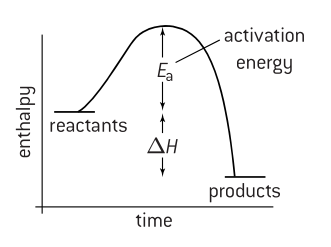
\includegraphics[scale=0.9]{activation_energy}
\caption{Graphe de l'énergie d'activation}
\end{figure}

\vspace{0.5em}
\textbf{Distribution de Maxwell-Boltzmann:}
Seulement une fraction petite des particules on une énergie cinétique suffisante pour faire la réaction, le catalyseur augmente la fraction qui sont au dessus de l'énergie d'activation et la température change la courbe elle-même (voir les graphes).

\begin{figure}[H]
\centering
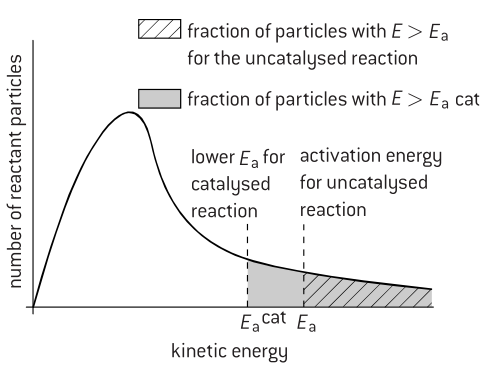
\includegraphics[scale=0.8]{maxwell-boltzmann}
\caption{Distribution normale qui doit être dessinée}
\end{figure}

\begin{figure}[H]
\centering
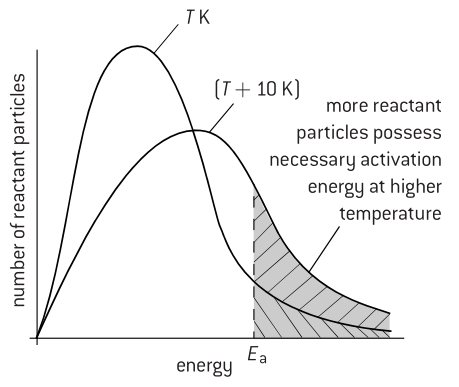
\includegraphics[scale=0.8]{maxwell-boltzmann_temperature}
\caption{Changement de la courbe à cause d'une augmentation de la température}
\end{figure}
\pagebreak

\section{Équilibre}
\pagebreak

\section{Acides et Bases}
\pagebreak

\section{Processus Redox}
\pagebreak

\section{Chimie Organique}
\pagebreak

\section{Mesure et Traitement des Données}
\pagebreak

\end{document}